\documentclass[a4paper,5p]{elsarticle}

\usepackage[utf8]{inputenc}
\usepackage[T5]{fontenc}
\usepackage{amsmath}
\usepackage{amssymb}
\usepackage{booktabs}
\usepackage{tabularx}
\usepackage{array}
\usepackage{graphicx}
\usepackage{xcolor}
\usepackage{dblfloatfix}
\usepackage{microtype}
\usepackage{xurl}
\usepackage[hidelinks]{hyperref}

\journal{Image and Vision Computing}

\newcommand{\method}{PACE-Seg}
\newcommand{\miou}{mIoU}
\newcommand{\etal}{et al.}
\setlength{\emergencystretch}{2em}
\hfuzz=3pt

\begin{document}

\begin{frontmatter}

\title{When Does Calibrated Capacity Routing Pay Off on Edge Accelerators? A Measured-Cost Analysis of Elastic Semantic Segmentation}

% TODO(author): confirm author list/order, full affiliation postal addresses, and corresponding e-mail.
\author[aff1]{Dũng Nguyễn\corref{cor1}}
\ead{[CORRESPONDING-AUTHOR-EMAIL]}
\cortext[cor1]{Corresponding author.}
\affiliation[aff1]{organization={[DEPARTMENT, INSTITUTION]},
            addressline={[STREET ADDRESS]},
            city={[CITY]},
            postcode={[POSTCODE]},
            country={[COUNTRY]}}

\begin{abstract}
Input-adaptive capacity routing promises to spend computation only where an image needs it, but on edge accelerators its benefit must be weighed against the cost of probing, deciding, and switching engines. We study this trade-off with \method{}, an elastic semantic-segmentation model whose four capacities are exported as static TensorRT and Hailo-8 engines, and a family of budget-aware routers driven by one entropy probe. Measuring every candidate, every route, and every static deployment with the same harness on four edge devices, we find that a FLOPs-proportional proxy misestimates feasibility (a $110.2\times$ compute range becomes a $12$--$18\times$ measured latency range); that the largest elastic capacity is 1.0 \miou{} points below the same architecture trained alone on Cityscapes and 2.0 points below on ACDC; and that routing under a hard measured budget outperforms rank escalation by 2.9 \miou{} points (95\% CI 2.5--3.3; nested 1.8--3.3) while a three-threshold scalar router matches candidate-specific calibration. Against static deployment charged its own direct latency, however, routing never wins on either a TensorRT GPU or a Hailo-8 (2.6 and 7.4--9.2 points below the best feasible static model), because the probe, decision, and engine switch cost 0.7--2.7 and 38--47~ms per frame. A break-even analysis shows routing pays off only under mean-cost budgets and when this overhead stays below about 1.3 and 4.3~ms, which we turn into design guidance for adaptive inference on edge accelerators.
\end{abstract}

\begin{keyword}
semantic segmentation \sep dynamic inference \sep edge acceleration \sep hardware-aware deployment \sep uncertainty calibration \sep negative results
\end{keyword}

\end{frontmatter}

%======================================================================
\section{Introduction}
\label{sec:introduction}

\begin{table*}[!t]
\centering
\caption{Mechanism-level positioning relative to representative primary work. Entries summarize the stated operating mechanism rather than rank methods or claim exhaustive coverage. ``Complete route'' includes the probe, risk computation, policy decision, backend dispatch or activation, and any additional candidate inference.}
\label{tab:related-positioning}
\footnotesize
\setlength{\tabcolsep}{4pt}
\begin{tabularx}{\textwidth}{@{}lllll>{\raggedright\arraybackslash}X@{}}
\toprule
Method & Candidates & Selection & Cost & Risk & Budget; deployed form \\
\midrule
Once-for-All~\cite{cai2020ofa} & Elastic subnetworks & Design & Latency predictor & None & Design constraint; static subnet \\
SlimSeg~\cite{xue2022slimseg} & Slimmable widths & Configured & Efficiency setting & None & No hard measured budget; static width \\
MESS~\cite{kouris2022mess} & Multi-exit network & Per image & Exit latency & Exit confidence & No complete-route constraint; multi-exit graph \\
Dynamic Routing~\cite{li2020dynamic} & Multi-scale paths & Per image & Compute penalty & Learned gates & No measured accelerator constraint; dynamic paths \\
AutoSegEdge~\cite{dou2023autosegedge} & Searched architecture & Design & FLOPs + device latency & None & Search constraint; static architecture \\
\method{} & Four elastic capacities & Per image & Measured complete route & Candidate-specific error & Hard measured budget; static compiled engines \\
\bottomrule
\end{tabularx}
\end{table*}

A vehicle or mobile robot that segments its surroundings on an embedded accelerator must return a label map within a latency budget, while its input varies from clear daylight to fog, rain, snow, and night. Input-adaptive inference offers an appealing answer: run a small model on easy frames and a large one only when needed. Elastic networks make the candidate models cheap to obtain from one set of weights~\cite{yu2019usnet,cai2020ofa}, and many dynamic-inference methods report substantial compute savings~\cite{han2022dynamic}.

Whether these savings survive deployment on an edge accelerator is less clear. Compute counts such as FLOPs do not translate proportionally into latency~\cite{li2021hwnasbench}, and an adaptive pipeline adds work a static deployment never pays: a probe to estimate difficulty, a decision, and on some accelerators a switch between compiled engines. Most dynamic-inference studies compare against static baselines in FLOPs or with idealized costs, so the question of when routing actually beats simply running the best static model that fits the budget is rarely answered with measurements.

This paper answers that question for elastic semantic segmentation. We build \method{}, whose four capacities (tiny to large, 384$\times$192 to 1024$\times$512 pixels, width$\times$height) are exported as static engines, and a family of routers that share one entropy probe but differ in how they use it: rank escalation, the same with a hard budget, a tuned three-threshold scalar router, and candidate-specific calibrated risk. Every candidate, route, and static deployment is timed with one harness on a TensorRT GPU and a Hailo-8 accelerator, and segmentation quality is measured with compiled engines as well as in replay.

We ask three questions. RQ1: does a FLOPs-proportional proxy reproduce measured feasibility? RQ2: does shared elastic training preserve the quality of the largest capacity, compared with the same architecture trained alone? RQ3: when all costs are measured, which routing ingredients matter, and does routing beat static deployment? Our answers are: no, the proxy overstates the latency range by six to nine times; shared training costs the largest capacity 1.0 \miou{} points on Cityscapes and 2.0 points on ACDC, a modest price for obtaining three smaller capacities from the same weights; and the hard budget and threshold tuning matter while candidate-specific calibration does not, but static deployment wins under per-frame budgets and at the measured overheads. A break-even analysis then quantifies how small the routing overhead must become for routing to pay off.

The contributions are:
\begin{enumerate}
    \item a measurement methodology that charges adaptive routes and static deployments their own costs from one harness and one timer boundary, applied to four edge devices including a Hailo-8;
    \item an ablation that separates the hard budget, threshold tuning, and candidate-specific calibration in budget-aware routing, with image-level and nested bootstrap intervals;
    \item a quantified negative result and break-even analysis showing when capacity routing does and does not pay off on edge accelerators;
    \item compiled-engine accuracy for TensorRT FP16 and Hailo-8 INT8 and an on-device replay of the routing results; code and protocols are released.
\end{enumerate}

%======================================================================
\section{Related work}
\label{sec:related}

\begin{figure*}[t]
\centering
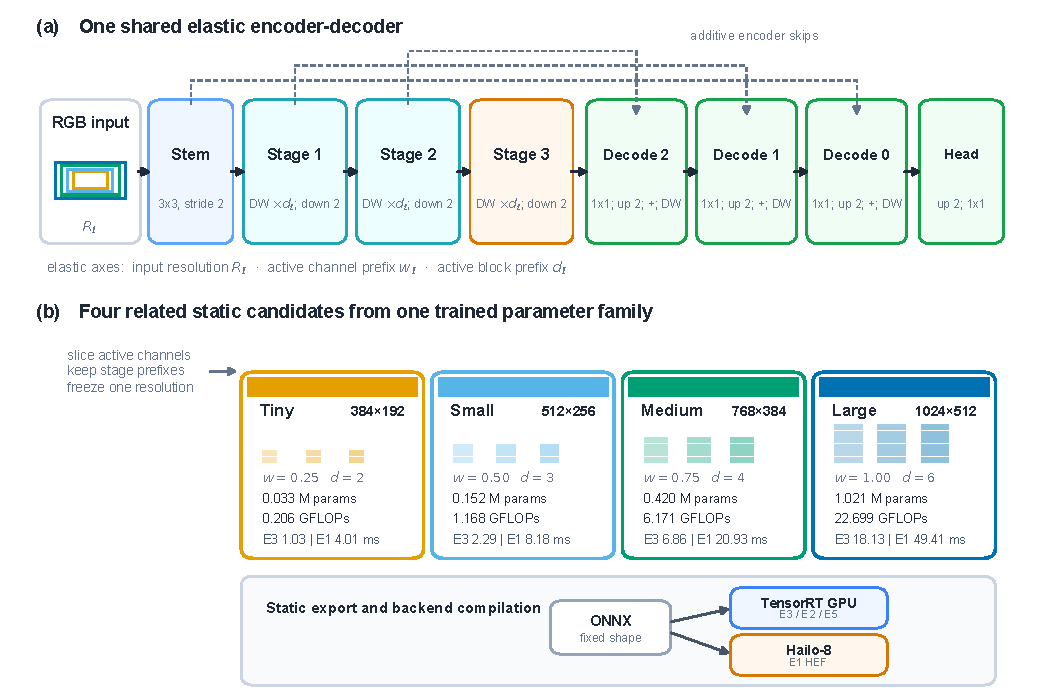
\includegraphics[width=\textwidth]{figures/fig2_architecture_v20.pdf}
\caption{(a) The shared elastic encoder--decoder. (b) The four static candidates exported from one trained supernet, with input size (width$\times$height), parameters, compute, and measured p95 latency on E3 and E1.}
\label{fig:arch}
\end{figure*}

\subsection{Efficient semantic segmentation}

Fully convolutional networks established dense end-to-end prediction~\cite{long2015fcn}, and pyramid pooling and atrous encoder--decoders raised accuracy at substantial computational cost~\cite{zhao2017pspnet,chen2018deeplabv3plus}. Real-time designs reduce that cost in several ways. ENet and ERFNet use early downsampling and factorized convolutions~\cite{paszke2016enet,romera2018erfnet}, ICNet cascades low- and high-resolution branches~\cite{zhao2018icnet}, and Fast-SCNN shares a learning-to-downsample module between a global feature extractor and a high-resolution path~\cite{poudel2019fastscnn}. Fast-SCNN serves as our matched-capacity comparator because it occupies a similar sub-million-parameter regime with the depthwise-separable operators that also underlie mobile classification networks~\cite{sandler2018mobilenetv2,howard2019mobilenetv3}.

Current real-time models are dominated by two-branch and multi-resolution designs. BiSeNet and BiSeNetV2 separate spatial detail from semantic context~\cite{yu2018bisenet,yu2021bisenetv2}, STDC replaces the extra spatial path with detail-guided training~\cite{fan2021stdc}, DDRNet maintains bilateral dual-resolution fusion~\cite{pan2023ddrnet}, and PIDNet adds a boundary branch inspired by PID control~\cite{xu2023pidnet}. SegFormer and OffSeg improve the accuracy--efficiency frontier through efficient attention and offset-based feature alignment~\cite{xie2021segformer,zhang2025offseg}. Despite their different mechanisms, these models share one deployment assumption: after compilation, every image passes through the same operating point. \method{} is complementary to this line. Any family of compilable candidates could replace its elastic encoder--decoder; we keep one family fixed so that routing effects are not confounded with architectural differences.

\subsection{Elastic and input-adaptive networks}

Slimmable networks train shared weights at several preset widths with switchable batch normalization, and US-Net extends this to arbitrary widths with the sandwich rule and in-place distillation~\cite{yu2019slimmable,yu2019usnet}. Once-for-All trains a broader depth--width--resolution--kernel space and extracts a specialized subnetwork for each target under a latency predictor~\cite{cai2020ofa}. SlimSeg brings slimmable training to segmentation with stepwise distillation~\cite{xue2022slimseg}. \method{} adopts the sandwich rule and in-place distillation, but freezes each capacity into a separate static graph instead of switching widths inside one dynamic model, which keeps the engines compatible with accelerators such as Hailo-8 that do not execute data-dependent control flow.

A related line adapts computation to each input. Early-exit classifiers such as BranchyNet and MSDNet stop at an intermediate predictor once confidence is sufficient~\cite{teerapittayanon2016branchynet,huang2018msdnet}, and SkipNet and BlockDrop learn per-input layer or block execution~\cite{wang2018skipnet,wu2018blockdrop}; Han~\etal{} survey these sample-, spatial-, and temporal-wise variants~\cite{han2022dynamic}. For dense prediction, Dynamic Routing selects scale-transform paths with learned gates~\cite{li2020dynamic}, Anytime Dense Prediction refines its output through confidence-adaptive exits~\cite{liu2022anytime}, and MESS chooses among the exits of a multi-exit segmentation network~\cite{kouris2022mess}. Most of these methods express cost through FLOPs or a soft training penalty and execute their adaptivity inside one graph. \method{} moves the decision outside the graph and constrains it by measured latency, at the price of coarser granularity: it chooses among four engines rather than among layers or exits.

\subsection{Hardware-aware design and latency modelling}

MnasNet made measured on-device latency a search objective~\cite{tan2019mnasnet}, and ProxylessNAS and FBNet searched directly on target hardware or through latency lookup tables~\cite{cai2019proxylessnas,wu2019fbnet}. FasterSeg, AutoSegEdge, multi-objective edge NAS, RealtimeSeg, and HARD bring platform cost into segmentation architecture design~\cite{chen2020fasterseg,dou2023autosegedge,dou2024multiobjective,li2023realtimeseg,kwon2024hard}. HW-NAS-Bench documented that FLOPs and measured latency diverge across devices~\cite{li2021hwnasbench}, and nn-Meter predicts kernel-level latency for unseen models~\cite{zhang2021nnmeter}. All of these use hardware cost to choose one architecture before deployment. \method{} uses cost at run time to restrict a fixed candidate set per device; because the set is small, every complete route can be measured directly and no latency predictor is needed. RQ1 accordingly evaluates only a proportional FLOPs proxy and makes no claim about learned predictors.

\subsection{Uncertainty and calibration under adverse conditions}

Monte Carlo dropout, deep ensembles, and aleatoric--epistemic decompositions estimate predictive uncertainty~\cite{gal2016dropout,lakshminarayanan2017ensembles,kendall2017uncertainties}, but require multiple passes or extra heads that are costly on edge accelerators. Modern networks are often miscalibrated~\cite{guo2017calibration}, and monotone post-hoc mappings such as histogram binning and isotonic regression are standard corrections~\cite{zadrozny2002isotonic}. Selective prediction asks whether a score ranks errors correctly and summarizes this with risk--coverage curves and AURC~\cite{geifman2017selective}; conformal risk control adds distribution-free guarantees under exchangeability~\cite{angelopoulos2024crc}. In segmentation, calibration degrades under domain shift and differs across model capacities~\cite{wang2023calibrating,dejorge2023reliability}. Foggy Cityscapes and Dark Zurich target fog and night~\cite{sakaridis2018foggy,sakaridis2019darkzurich}, and ACDC provides real fog, night, rain, and snow images with Cityscapes-compatible labels~\cite{sakaridis2021acdc}. \method{} uses a single-pass entropy score and a separate binned monotone calibrator per candidate; its estimates support risk-aware selection but provide no formal risk guarantee.

\subsection{Positioning}

Table~\ref{tab:related-positioning} compares the closest methods by how they construct candidates, when they select, and how they represent cost and risk. \method{} combines per-image selection, candidate-specific error estimates, and a budget defined by the measured complete accelerator route on static compiled engines. We use this combination as a test bed rather than as a proposed method: because every ingredient can be switched off and every cost is measured, it lets us ask which ingredients matter and whether the whole pipeline beats a static deployment timed in the same harness.

%======================================================================
\section{System under study}
\label{sec:method}

\subsection{Elastic candidate family}

\method{} is an encoder--decoder whose four capacities jointly vary width multiplier (0.25, 0.50, 0.75, 1.00), repeated-block depth (2, 3, 4, 6), and input resolution (384$\times$192, 512$\times$256, 768$\times$384, 1024$\times$512, width$\times$height, matching the 2:1 aspect of Cityscapes and ACDC). Capacities share convolutional weights through active-channel slicing and keep level-specific batch normalization~\cite{yu2019slimmable}; each exports as a fixed-shape ONNX graph and compiles to a static TensorRT or Hailo-8 engine.

\subsection{Training}

All capacities are trained together with the sandwich rule~\cite{yu2019usnet}: each step samples the smallest, the largest, and one intermediate level, each supervised by boundary-aware cross-entropy ($\lambda_b=1$), with in-place distillation from the detached largest level ($\alpha=0.5$, $T=1$)~\cite{hinton2015distilling}. Training uses 100,000 steps, batch 8, AdamW ($3\times10^{-4}$, weight decay $10^{-4}$), 500 warm-up steps with cosine decay, gradient clipping at 5.0, FP16 mixed precision, and training augmentation of random scaling (0.75--1.25), cropping, horizontal flipping, and colour jitter (brightness, contrast, and saturation 0.3). Three supernets are trained with seeds 0--2. As references, Fast-SCNN~\cite{poudel2019fastscnn} and the large \method{} architecture trained alone (no weight sharing or distillation) are each trained with three seeds and the same recipe.

\subsection{Probe and routing policies}

The tiny engine always runs first; its mean pixel entropy $s(x)$ is the probe. All routers use the same probe and differ only in how they map it to a capacity under a budget $B_h$:
\begin{itemize}
    \item \textbf{A (rank escalation):} a calibrated scalar risk $\hat r_\text{tiny}(x)$ selects the candidate at latency rank $\lfloor \hat r_\text{tiny}/\tau\rfloor$; no budget mask.
    \item \textbf{A-hard:} A with a feasibility mask; an infeasible choice is replaced by the most expensive feasible route.
    \item \textbf{T-hard:} three monotone thresholds on $s(x)$ fitted on the fit half to maximize fit-half \miou{} under the budget, with the same mask.
    \item \textbf{D (candidate-specific risk):} four binned monotone calibrators $g_\ell$~\cite{zadrozny2002isotonic} map $s(x)$ to per-candidate expected errors; D picks the cheapest feasible candidate meeting a target $\tau$, otherwise the lowest-risk feasible one.
\end{itemize}
The static references run one capacity alone: the best feasible static candidate (largest whose direct cost fits $B_h$) and, for mean-cost budgets, a random mixture of two adjacent static candidates.

%======================================================================
\section{Measurement methodology}
\label{sec:protocol}

\begin{figure}[!htb]
\centering
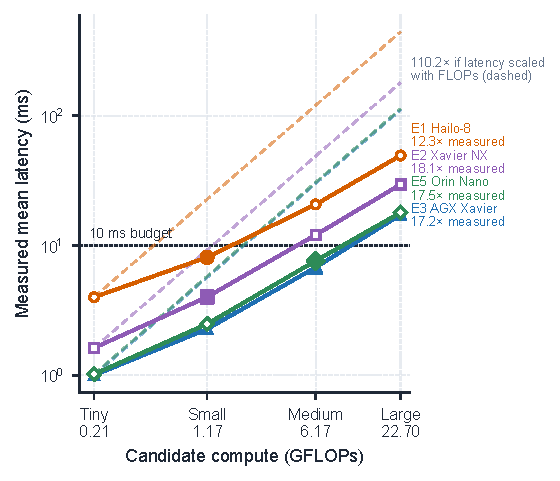
\includegraphics[width=\linewidth]{figures/fig5_flops_latency_v20.pdf}
\caption{Measured mean latency of the four capacities on four devices (solid) against the latency a FLOPs-proportional proxy anchored at tiny would predict (dashed). Filled markers: largest capacity within a 10~ms budget.}
\label{fig:flops}
\end{figure}

\begin{figure*}[!t]
\centering
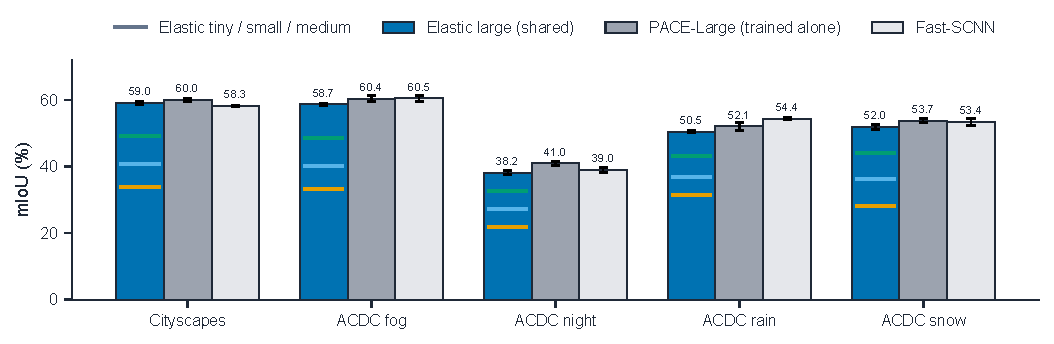
\includegraphics[width=0.82\textwidth]{figures/fig6_rq2_shared_vs_alone_v20.pdf}
\caption{Absolute \miou{} of the largest elastic capacity (shared training), the same architecture trained alone (PACE-Large), and Fast-SCNN, mean $\pm$ standard deviation over three seeds. Short ticks on the elastic bars mark the tiny (orange), small (light blue), and medium (green) capacities of the same supernets.}
\label{fig:rq2}
\end{figure*}

\subsection{Devices and compiled engines}

Table~\ref{tab:devices} lists the four devices. TensorRT engines are FP16; Hailo-8 HEFs are INT8, quantized with 200 real fit-half images. Accuracy of every compiled engine is measured on the held-out images (Section~\ref{sec:compiled}).

\begin{table}[t]
\centering
\caption{Edge devices and toolchains. E1 and E3 carry the routing measurements; all four carry the candidate-only latency table of RQ1.}
\label{tab:devices}
\small
\footnotesize
\begin{tabularx}{\linewidth}{@{}l>{\raggedright\arraybackslash}Xl@{}}
\toprule
ID & Device & Runtime, precision \\
\midrule
E1 & Raspberry Pi 5 + Hailo-8 & HailoRT 4.23, INT8 \\
E2 & Jetson Xavier NX & TensorRT (R35.4.1), FP16 \\
E3 & Jetson AGX Xavier (MAXN) & TensorRT 8.5.2, FP16 \\
E5 & Jetson Orin Nano & TensorRT, FP16 \\
\bottomrule
\end{tabularx}
\end{table}

\subsection{One harness for routes and static deployments}

Route cost $C_h(\ell)$ and static cost $S_h(\ell)$ are measured in the same process, with the same engines, inputs, and timer boundary: from handing preprocessed host tensors to the runtime to the synchronized output of the returned prediction. A route runs the tiny engine, computes entropy and the policy decision, and, unless tiny is selected, runs the selected engine; a static deployment runs only its engine. On E1 we report both explicit network-group activation and the HailoRT model scheduler, and both FLOAT32 and UINT8 vstreams. Each class uses 50 warm-up and 500 timed iterations; medians, p95, and p99 are reported. Candidate-only latency for RQ1 uses the trtexec/hailortcli protocol on all four devices.

\subsection{Data, splits, and statistics}

Cityscapes provides 2,975 training and 500 validation images~\cite{cordts2016cityscapes}, and ACDC provides 1,600 training and 406 validation images across fog, night, rain, and snow~\cite{sakaridis2021acdc}; both use the 19 Cityscapes training classes, and all models are trained on the training sets. Validation images are split by alternating index into fit and held-out halves; calibrators, thresholds, risk targets, and operating points use only the fit half. Budgets are the union of the measured route and static costs of a device. An operating cell is (run, device, split, budget). Intervals are image-level bootstrap and nested bootstrap (refitting on resampled fit halves); a leave-one-condition-out analysis withholds each condition from calibration.

%======================================================================
\section{Results}
\label{sec:results}

\begin{figure*}[t]
\centering
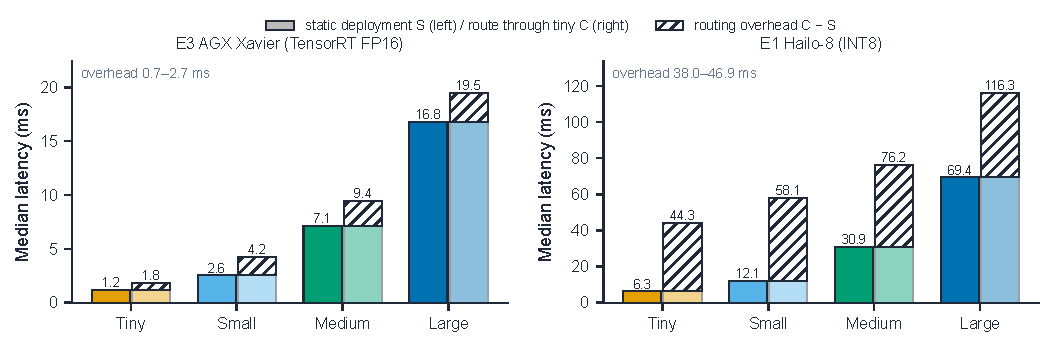
\includegraphics[width=\textwidth]{figures/fig11_route_vs_static_v20.pdf}
\caption{Same-harness median latency of each capacity deployed statically (left bars) and reached through the tiny probe (right bars). Hatched: routing overhead. E3 returns logits; E1 uses explicit network-group activation with FLOAT32 vstreams.}
\label{fig:routestatic}
\end{figure*}

\begin{figure*}[t]
\centering
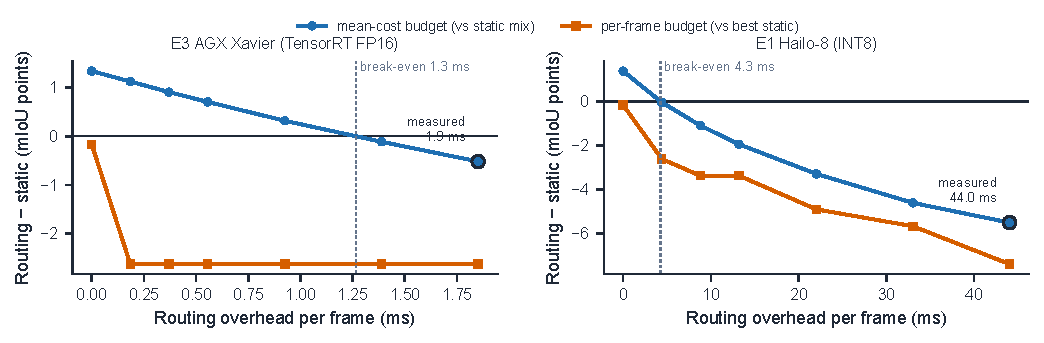
\includegraphics[width=\textwidth]{figures/fig12_breakeven_v20.pdf}
\caption{Routing minus static \miou{} as the measured routing overhead is scaled from zero to its measured value (circle). Blue: mean-cost budgets against static mixing; orange: per-frame budgets against the best feasible static model. Dotted: break-even overhead.}
\label{fig:breakeven}
\end{figure*}

\subsection{RQ1: FLOPs versus measured feasibility}

The four capacities span 0.21 to 22.70 GFLOPs, a $110.2\times$ range. Measured mean latency spans only $12.3\times$ on the Hailo-8 (4.0 to 49.3~ms), $17.2\times$ on E3 (1.0 to 17.2~ms), $17.5\times$ on E5 (1.0 to 18.0~ms), and $18.1\times$ on E2 (1.6 to 29.5~ms) (Fig.~\ref{fig:flops}). A proxy anchored at tiny therefore predicts 110~ms for large on E3 and 441~ms on E1, overstating the measured value by $6$--$9\times$, and under a 10~ms budget it would rule out medium on E3 and E5 and small on E1, all of which measurement shows to fit. The small candidates are memory- and launch-bound, so their latency falls far less than their compute; feasibility must come from measured tables.


\subsection{RQ2: shared training versus standalone training}

Fig.~\ref{fig:rq2} compares the largest elastic capacity with the same architecture trained alone (PACE-Large) and with Fast-SCNN, each over three seeds. Shared training costs the large capacity 1.0 \miou{} points on Cityscapes ($59.0\pm0.3$ vs $60.0\pm0.5$) and 2.0 points on the ACDC mean ($49.8\pm0.1$ vs $51.8\pm0.7$); the gap is largest at night ($-2.8$) and 1.6--1.7 points under fog, rain, and snow. Against Fast-SCNN, the elastic large capacity is 0.7 points better on Cityscapes and 2.0 points worse on the ACDC mean, so it sits within the accuracy range of real-time single-capacity models while also providing tiny, small, and medium capacities (33.8, 40.8, and 49.3 \miou{} on Cityscapes) from the same weights. The cost of weight sharing therefore grows under adverse conditions, which is where the routers of RQ3 would most want the large capacity.

\subsection{RQ3a: which routing ingredients matter}
\label{sec:rq3}

Table~\ref{tab:ablation} separates the routing ingredients, pooled over three supernets, two devices, five splits, and the budget grid. Adding a hard budget to rank escalation already gains 0.5 points; candidate-specific risk (D) adds 1.4 points over A-hard (nested CI 1.0--1.7) and never loses a cell. The same gain is obtained without candidate-specific calibration: the three-threshold scalar router T-hard is statistically indistinguishable from D ($-0.03$ points, CI $-0.11$ to $+0.09$) at 1\% lower cost, and pooling the four calibrators changes nothing. The ordering is unchanged at p95 and p99 costs and under leave-one-condition-out calibration (D beats A-hard by 1.6 points with no losing cell). Per-candidate calibrators are well calibrated (Fig.~S5; mean absolute error 0.02--0.03 in pixel error), so the absence of a gain is not caused by poor calibration: with one scalar probe, a monotone threshold rule already captures the information the calibrators add.

\begin{table}[t]
\centering
\caption{Routing ablation (median costs, \miou{} points). $^{\dagger}$Fair cells only: budgets where both policies are feasible. W/T/L: operating cells won, tied, and lost. Nested intervals refit calibrators, risk grid, and operating points on resampled fit halves.}
\label{tab:ablation}
\footnotesize
\setlength{\tabcolsep}{3pt}
\begin{tabular*}{\linewidth}{@{\extracolsep{\fill}}lrccc@{}}
\toprule
Comparison & $\Delta$ & 95\% CI & Nested CI & W/T/L \\
\midrule
D $-$ A$^{\dagger}$ & $+2.87$ & 2.52, 3.26 & 1.85, 3.28 & 54/6/2 \\
A-hard $-$ A$^{\dagger}$ & $+0.47$ & -- & -- & 22/38/2 \\
D $-$ A-hard & $+1.41$ & 1.19, 1.63 & 0.99, 1.70 & 48/72/0 \\
T-hard $-$ A-hard & $+1.44$ & -- & -- & 46/68/6 \\
D $-$ T-hard & $-0.03$ & $-0.11$, 0.09 & -- & 16/80/24 \\
\bottomrule
\end{tabular*}
\end{table}

\subsection{RQ3b: routing versus static deployment}

Fig.~\ref{fig:routestatic} shows why routing loses once static deployment is charged its own latency. On E3 a route costs 0.7~ms more than the static engine it ends in for tiny and 2.7~ms more for large; on E1 the overhead is 38--47~ms, almost the full latency of the large engine, and it does not shrink with the HailoRT scheduler or UINT8 vstreams. Under per-frame budgets the best feasible static model beats D by 2.6 points on E3 (CI $-2.7$ to $-2.4$; 0 wins, 61 ties, 59 losses) and by 7.4 (FLOAT32) to 9.2 (UINT8) points on E1 (0 wins); T-hard behaves identically. Under mean-cost budgets the fairer reference is a random mixture of two adjacent static models with the same mean cost; candidate-specific routing still loses by 0.3--0.5 points on E3 and 5.5--6.3 points on E1. At the lowest budgets of each device no route is feasible at all, because the cheapest route (tiny plus probe) already exceeds the static tiny engine.

\subsection{Break-even overhead}

To ask how much the overhead would have to shrink, we scale the measured per-capacity overhead by $\alpha\in[0,1]$ and repeat the comparison (Fig.~\ref{fig:breakeven}). With zero overhead, routing would gain 1.3--1.4 points over static mixing under mean-cost budgets on both devices. The gain vanishes at 1.3~ms on E3 (measured: 1.9~ms) and 4.3~ms on E1 (measured: 44~ms). Under per-frame budgets routing never wins, even at zero overhead ($-0.16$ points): any per-frame cap forces the router to stay at or below the capacity that the static model already uses, so it can only lose.

\subsection{Compiled-engine accuracy and on-device replay}
\label{sec:compiled}

Compiled TensorRT FP16 engines reproduce PyTorch within $\pm0.02$ points on every capacity and split, with 99.7--100\% pixel agreement and a probe-entropy error below $2\times10^{-4}$. Hailo-8 INT8 engines lose up to 1.6 points on tiny (pixel agreement down to 87\% at night) and at most 0.5 points on large; the probe entropy deviates by 0.012--0.035 on average but keeps a rank correlation of at least 0.88. Replaying Run A with the on-device predictions and probe scores leaves every conclusion unchanged: on E3 D differs from the PyTorch replay by 0.01 points, and on E1 D loses a further 0.6 points but still matches T-hard ($-0.06$) and trails static by 7.9 points.

%======================================================================
\section{Discussion}
\label{sec:discussion}

\subsection{Why static deployment wins here}

Routing can only pay off if choosing per image is worth more than its cost. The headroom is small: D is within 0.3 points of the ground-truth pixel-error oracle reference on the same probe, and even at zero overhead routing gains only 1.3--1.4 points over static mixing. Against that, every route pays for the tiny engine, the entropy and decision, and on the Hailo-8 a network-group switch that dominates the cost. Per-frame budgets remove the remaining room, because the static model can always run the largest capacity that the cap allows.

\subsection{When routing can pay off}

Routing becomes worthwhile when three conditions hold: the budget constrains mean rather than per-frame cost; the overhead stays below the break-even value (about 1.3~ms on E3 and 4.3~ms on E1 here); and the candidates differ enough per image to leave headroom. Designs that reuse the probe computation inside the selected candidate, keep all candidates resident without switching (multi-context compilation on Hailo, one engine with shared early layers on TensorRT), or route among models with more complementary errors attack exactly these terms. For a fixed per-frame budget, a static model of the largest feasible capacity is the stronger baseline and should be reported.

\subsection{Limitations}

We study two datasets (Cityscapes and ACDC) and an alternating-index fit/held-out split; compiled accuracy is measured for one of three supernets; energy is not measured; and accuracy under routing is obtained by replaying recorded predictions with measured costs rather than in a closed-loop deployment. The routing conclusions are drawn on one entropy probe and four candidates.

%======================================================================
\section{Conclusion}
\label{sec:conclusion}

We measured when calibrated capacity routing pays off for elastic semantic segmentation on edge accelerators. FLOPs misstate the latency range of the candidates by six to nine times, so feasibility must be measured. Shared elastic training costs the largest capacity 1.0 \miou{} points on Cityscapes and 2.0 on ACDC relative to training it alone. Among routers, a hard measured budget is what matters: it lifts routing 2.9 points over rank escalation, and a three-threshold scalar router matches candidate-specific calibration. Charged its own latency, however, static deployment beats routing on both a TensorRT GPU and a Hailo-8, and routing only breaks even under mean-cost budgets when its overhead falls below about 1.3 and 4.3~ms. Adaptive-inference studies on edge hardware should therefore report a static baseline timed in the same harness and the break-even overhead of their routing pipeline.

\section*{CRediT authorship contribution statement}

% TODO(author): adjust roles if co-authors are added.
\textbf{Dũng Nguyễn:} Conceptualization, Methodology, Software, Validation, Formal analysis, Investigation, Data curation, Visualization, Writing -- original draft, Writing -- review \& editing.

\section*{Declaration of competing interest}

% TODO(author): confirm.
The authors declare that they have no known competing financial interests or personal relationships that could have appeared to influence the work reported in this paper.

\section*{Funding}

% TODO(author): funder names and grant numbers, or the standard no-funding sentence.
[FUNDING STATEMENT TO BE PROVIDED.]

\section*{Data availability}

Code, measurement protocols, and result artifacts are available at [REPOSITORY URL OR DOI]. Cityscapes and ACDC are available from their providers under their licences and are not redistributed.

\section*{Acknowledgements}

[ACKNOWLEDGEMENTS TO BE PROVIDED.]

\section*{Declaration of generative AI and AI-assisted technologies in the manuscript preparation process}

During the preparation of this work the author used Claude (Anthropic) in order to assist with language editing, manuscript structuring, LaTeX formatting, analysis scripts, and scripts that render figures from the recorded experimental results. After using this tool, the author reviewed and edited the content as needed and takes full responsibility for the content of the published article.

\bibliographystyle{elsarticle-num}
\bibliography{references}

\end{document}
